\documentclass[a4paper,12pt]{article} % добавить leqno в [] для нумерации слева
\usepackage[a4paper,top=1.3cm,bottom=2cm,left=1.5cm,right=1.5cm,marginparwidth=0.75cm]{geometry}
%%% Работа с русским языком
\usepackage{cmap}					% поиск в PDF
\usepackage[warn]{mathtext} 		% русские буквы в фомулах
\usepackage[T2A]{fontenc}			% кодировка
\usepackage[utf8]{inputenc}			% кодировка исходного текста
\usepackage[english,russian]{babel}	% локализация и переносы
\usepackage{physics}
\usepackage{multirow}

%%% Нормальное размещение таблиц (писать [H] в окружении таблицы)
\usepackage{float}
\restylefloat{table}

\usepackage{graphicx}

\usepackage{wrapfig}
\usepackage{tabularx}

\usepackage{hyperref}
\usepackage[rgb]{xcolor}
\hypersetup{
	colorlinks=true,urlcolor=blue
}

%%% Дополнительная работа с математикой
\usepackage{amsmath,amsfonts,amssymb,amsthm,mathtools} % AMS
\usepackage{icomma} % "Умная" запятая: $0,2$ --- число, $0, 2$ --- перечисление

%% Номера формул
%\mathtoolsset{showonlyrefs=true} % Показывать номера только у тех формул, на которые есть \eqref{} в тексте.

%% Шрифты
\usepackage{euscript}	 % Шрифт Евклид
\usepackage{mathrsfs} % Красивый матшрифт
\usepackage{pgfplots}
\pgfplotsset{compat=1.9}

%% Свои команды
\DeclareMathOperator{\sgn}{\mathop{sgn}}

%% Перенос знаков в формулах (по Львовскому)
\newcommand*{\hm}[1]{#1\nobreak\discretionary{}
	{\hbox{$\mathsurround=0pt #1$}}{}}

\date{\today}

\begin{document}

\begin{titlepage}
	\begin{center}
		{\large МОСКОВСКИЙ ФИЗИКО-ТЕХНИЧЕСКИЙ ИНСТИТУТ (НАЦИОНАЛЬНЫЙ ИССЛЕДОВАТЕЛЬСКИЙ УНИВЕРСИТЕТ)}
	\end{center}
	\begin{center}
		{\large Физтех-школа аэрокосмических технологий}
	\end{center}
	\begin{figure}[h]
    		\centering
    		
\includegraphics[width=0.7\textwidth]{MIPT.jpg}
    		\label{setup}
	\end{figure}
	
	\vspace{3cm}
	{\huge
		\begin{center}
			{\bf Лабораторная работа 4.2.1}\\
			Кольца Ньютона
		\end{center}
	}
	\vspace{1cm}
	\begin{center}
		{\large Пазов Тенгиз \\
                    Симухин Егор \\
			\vspace{0.2cm}
			Б03-302}
	\end{center}
	\vspace{8cm}
	\begin{center}
		Февраль 2025
	\end{center}
\end{titlepage}

\section{Введение}
\section*{Цель работы}
Познакомиться с явлением интерференции в тонких
плёнках (полосы равной толщины) на примере колец Ньютона и с
методикой интерференционных измерений кривизны стеклянной поверхности.
\section{Экспериментальная установка}
\begin{figure}[h]
    \centering
    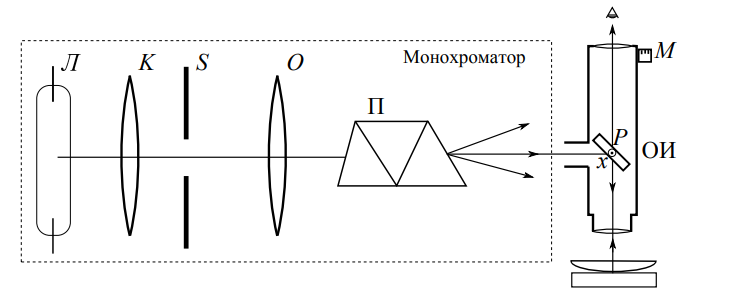
\includegraphics[width=0.7\textwidth]{установка.png}
    \caption{Схема экспериментальной установки}
    \label{setup}
\end{figure}
Схема экспериментальной установки приведена на рис. 1. Опыт выполняется с помощью измерительного
микроскопа. На столике микроскопа помещается держатель с пластинкой чёрного стекла. На пластинке лежит исследуемая линза.
Источником света служит ртутная лампа, находящаяся в защитном кожухе. Для получения монохроматического света применяется
призменный монохроматор, состоящий из конденсора K, коллиматора (щель S и объектив O) и призмы прямого зрения П. Эти устройства с помощью рейтеров располагаются на оптической скамье. Свет от
монохроматора попадает на опак-иллюминатор (ОИ), расположенный
между окуляром и объективом микроскопа — специальное устройство
для освещения объекта при работе в отражённом свете. Внутри опакиллюминатора находится полупрозрачная пластинка P, наклоненная
под углом 45◦ к оптической оси микроскопа. Свет частично отражается от этой пластинки, проходит через объектив микроскопа и попадает
на исследуемый объект. Пластинка может поворачиваться вокруг горизонтальной оси x, а опак-иллюминатор — вокруг вертикальной оси.
Столик микроскопа может перемещаться в двух взаимно перпендикулярных направлениях с помощью винтов препаратоводителя. Отсчетный крест окулярной шкалы перемещается перпендикулярно оптической оси микроскопа с помощью микрометрического винта.
Оптическая схема монохроматора позволяет получить в плоскости
входного окна опак-иллюминатора достаточно хорошо разделённые линии спектра ртутной лампы. Изображение щели S фокусируется на поверхность линзы объективом микроскопа, и в том же месте находится
плоскость наблюдения микроскопа, т. е. точка источника и точка наблюдения интерференции совпадают. Картина интерференции как и в
случае расположения пластинки сверху, так и в данном случае не зависит от коэффициента преломления линзы и определяется величиной
зазора между нижней поверхностью линзы и стеклянной пластинкой.
Рекомендуется сначала настроить микроскоп на кольца Ньютона в
белом свете (свете ртутной лампы), а затем после выделения монохроматором зелёной линии провести измерения в монохроматическом свете.
\section{Теоретические сведения}

Явление \textit{интерференции} возникает при падении двух или более когерентных электромагнитных волн~-- волн, разность фаз которых постоянна во времени и которые при сложении дают колебания постоянной частоты. Легче всего интерференция наблюдается при сложении двух монохроматических световых волн, исходящих изначально от одного источника. Интенсивность результирующей волны $I$ при этом определяется выражением
\begin{equation} \label{interference}
    I = 2I_0 \left( 1 + \cos \frac{2\pi}{\lambda}\Delta \right),
\end{equation}
где $I_0$~-- амплитуда интерферирующих волн, $\lambda$~-- длина волны, $\Delta = n_1r_1 - n_2r_2$~-- оптическая разность хода. Из \eqref{interference} видно, что максимум интенсивности достигается, когда в разность хода укладывается целое число длин волн, т.\,е.
\begin{equation}\label{maxInt}
    \Delta = m\lambda,\quad m \in \mathbb{N}.
\end{equation}
Для условия минимумов аналогично получаем
\begin{equation}\label{minInt}
    \Delta = (m + \frac{1}{2})\lambda,\quad m \in \mathbb{N}.
\end{equation}

\textbf{Кольца Ньютона}~-- классический опыт по наблюдению интерференции, возникающей при сложении волн, отражённых от границ тонкой воздушной прослойки между сферической поверхностями линзы и тонкой стеклянной пластинки (см. рис. \ref{NewtonRings}). При нормальном падении света интерференционная картина локализована на сферической поверхности линзы и состоит из полос равной толщины.
%\begin{figure}[h]
    %\centering
   % \includegraphics[width=0.5\textwidth]{NewtonRings.png}
  %  \caption{Схема наблюдения колец Ньютона}
 %   \label{NewtonRings}
%\end{figure}
Оптической разностью хода в данном случае является удвоенная толщина воздушной прослойки $2d$. Для точки сферической поверхности на расстоянии $r$ от оси системы $R^2 = r^2 + (R - d)^2$. Если линза тонкая, т.\,е. $R\gg r$, то $d = r^2/2R$. При преломлении световой волны на границе воздух-стелко фаза колебаний изменяется на $\pi$, откуда оптическая разность хода
\begin{equation}\label{strokeDiff}
    \Delta = 2d + \frac{\lambda}{2} = \frac{r^2}{R} + \frac{\lambda}{2}.
\end{equation}

Из условия интерференционного минимума \eqref{minInt} и \eqref{strokeDiff} получаем радиусы тёмных колец:
\begin{equation}\label{DarthRadius}
    r_m = \sqrt{2mR\lambda}.
\end{equation}
Аналогично, из \eqref{maxInt} получаются радиусы светлых колец:
\begin{equation}
    r'_m = \sqrt{(2m-1)R\lambda}.
\end{equation}

\section{Ход работы}
а)Вращая окулярный микрометрический винт, убедитесь, что перекрестие проходит через центр центрального тёмного пятна, и что поле зрения освещено симметрично слева и справа от центра.
Посмотрите, как влияет на освещённость поля зрения перемещение объектива О вдоль оптической скамьи.\\
б) Установите перекрестие на середину какого-либо достаточно удалённого от центра, но ещё отчётливо видимого тёмного кольца.
Снимите отсчёт по окулярной шкале: целые деления отсчитываются слева от риски, проходящей через окулярную шкалу, десятые и сотые доли деления — по окулярному микрометрическому винту М. Цена одного деления окулярной шкалы будет определена позже.
Для устранения ошибок, возникающих из-за люфта в микрометрическом винте, перекрестие следует подводить к каждому кольцу с одной стороны.
Перемещая перекрестие, последовательно устанавливайте его на середины тёмных и светлых колец и записывайте соответствующие показания окулярной шкалы и микрометра. После прохождения через центральное пятно продолжайте измерения, записывая возрастающие номера колец и координаты их диаметров. \\
Представим таблицу измерений радиусов колец.

установили на 9 кольцо. После этого двигаясь поочередно измеряли радиусы колей вплоть до начального.
\begin{figure}[h]
    \centering
    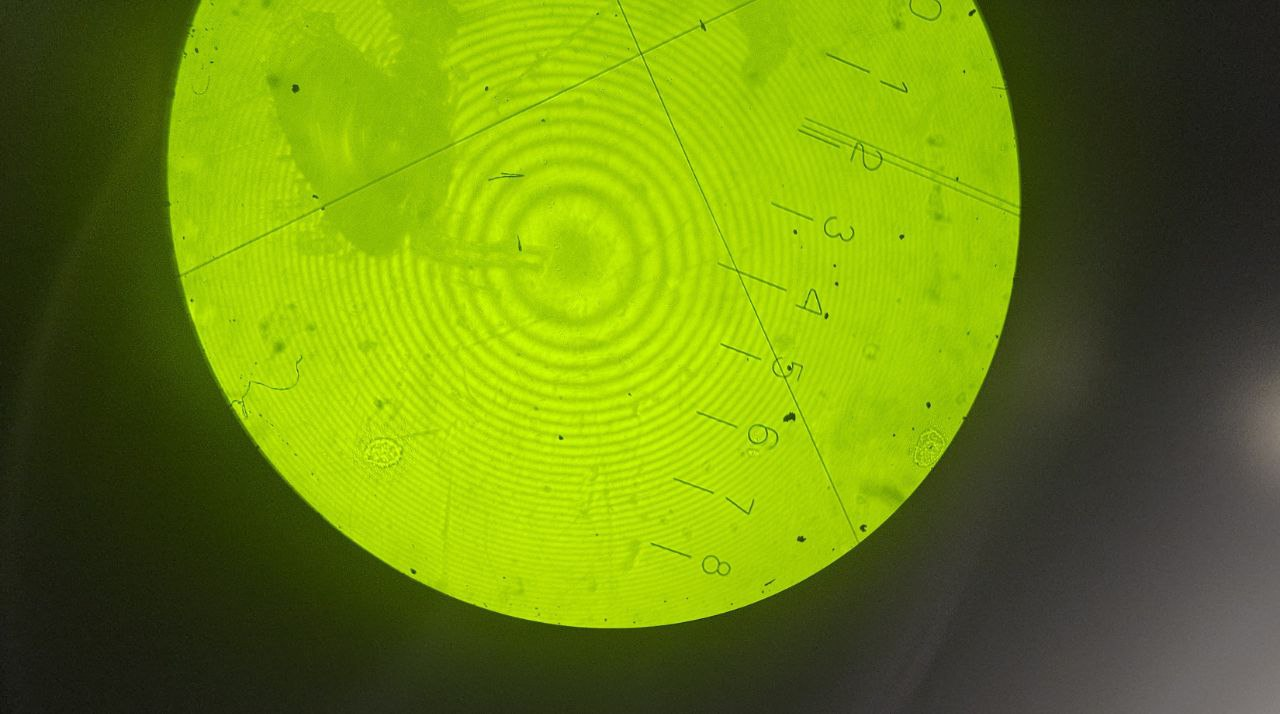
\includegraphics[width=0.7\textwidth]{пункт_б.jpg}
    \caption{Установка креста на самое дальнее чёткое кольцо}
    \label{setup}
\end{figure}
\\
в) Оцените диаметр пятна соприкосновения линзы со стеклянной пластинкой .\\
г) Пронаблюдали биения и в разделе "Результаты экспериментов" вычислили отношение длин волн.

\begin{figure}[h!!]
    \centering
    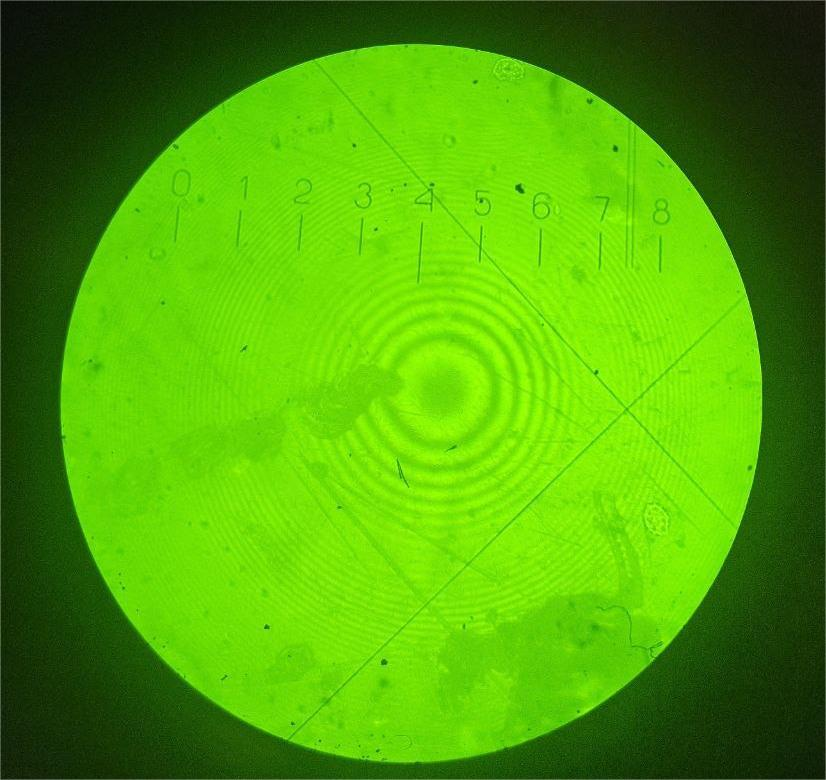
\includegraphics[width=0.5\textwidth]{биения.jpg}
    \caption{Наблюдение биений}
    \label{setup}
\end{figure}
д)
\begin{figure}[h]
    \centering
    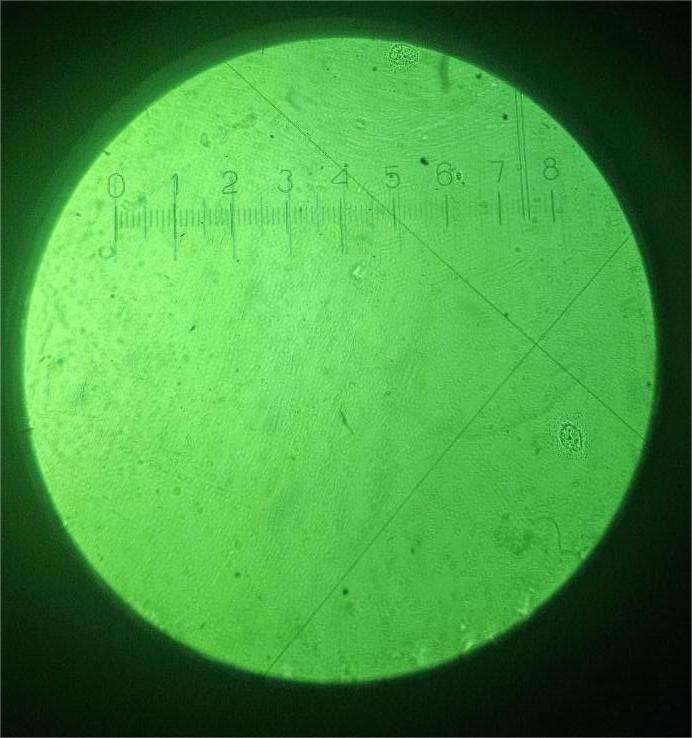
\includegraphics[width=0.5\textwidth]{калибровка.jpg}
    \caption{Калибровка}
    \label{setup}
\end{figure}
\section{Результаты экспериментов}
\begin{table}[H]
    \centering
    \begin{tabular}{|c|c|c|}
        \hline $m$ & $r_{m}^{2}$, мкм$^2$ & $r_{m}'^{2}$, мкм$^2$\\ \hline
        0 & 26,98 &  \\ \hline
        1 & 114,11 & 12,79 \\ \hline
        2 & 186,89 & 73,53 \\ \hline
        3 & 244,33 & 144,71 \\ \hline
        4 & 325,15 & 217,53 \\ \hline
        5 & 397,72 & 299,18 \\ \hline
        6 & 446,98 & 357,74 \\ \hline
        7 & 553,19 & 427,58 \\ \hline
        8 & 602,65 & 501,45 \\ \hline
        9 & 679,54 & 561,29 \\ \hline
        10 & 780,00 & 600,00 \\ \hline
        11 & 823,08 & 709,24 \\ \hline
    \end{tabular}
    \caption{Диаметры тёмных и светлых колец}
    \label{radi}
\end{table}
После юстировки экспериментальной установки были получены картины колец Ньютона
для каждого из фильтров. Картина для жёлто-зелёного фильтра изображена на рис. \ref{ringImage}. Для длины волны $\lambda = 579$ нм были измерены радиусы первых десяти тёмных колец в делениях измерительной шкалы. Затем было установлено, что одно деление измерительной шкалы совпадает с большим делением объектной шкалы и имеет длину 0,1 мм. 
\begin{figure}[h]
   \centering
   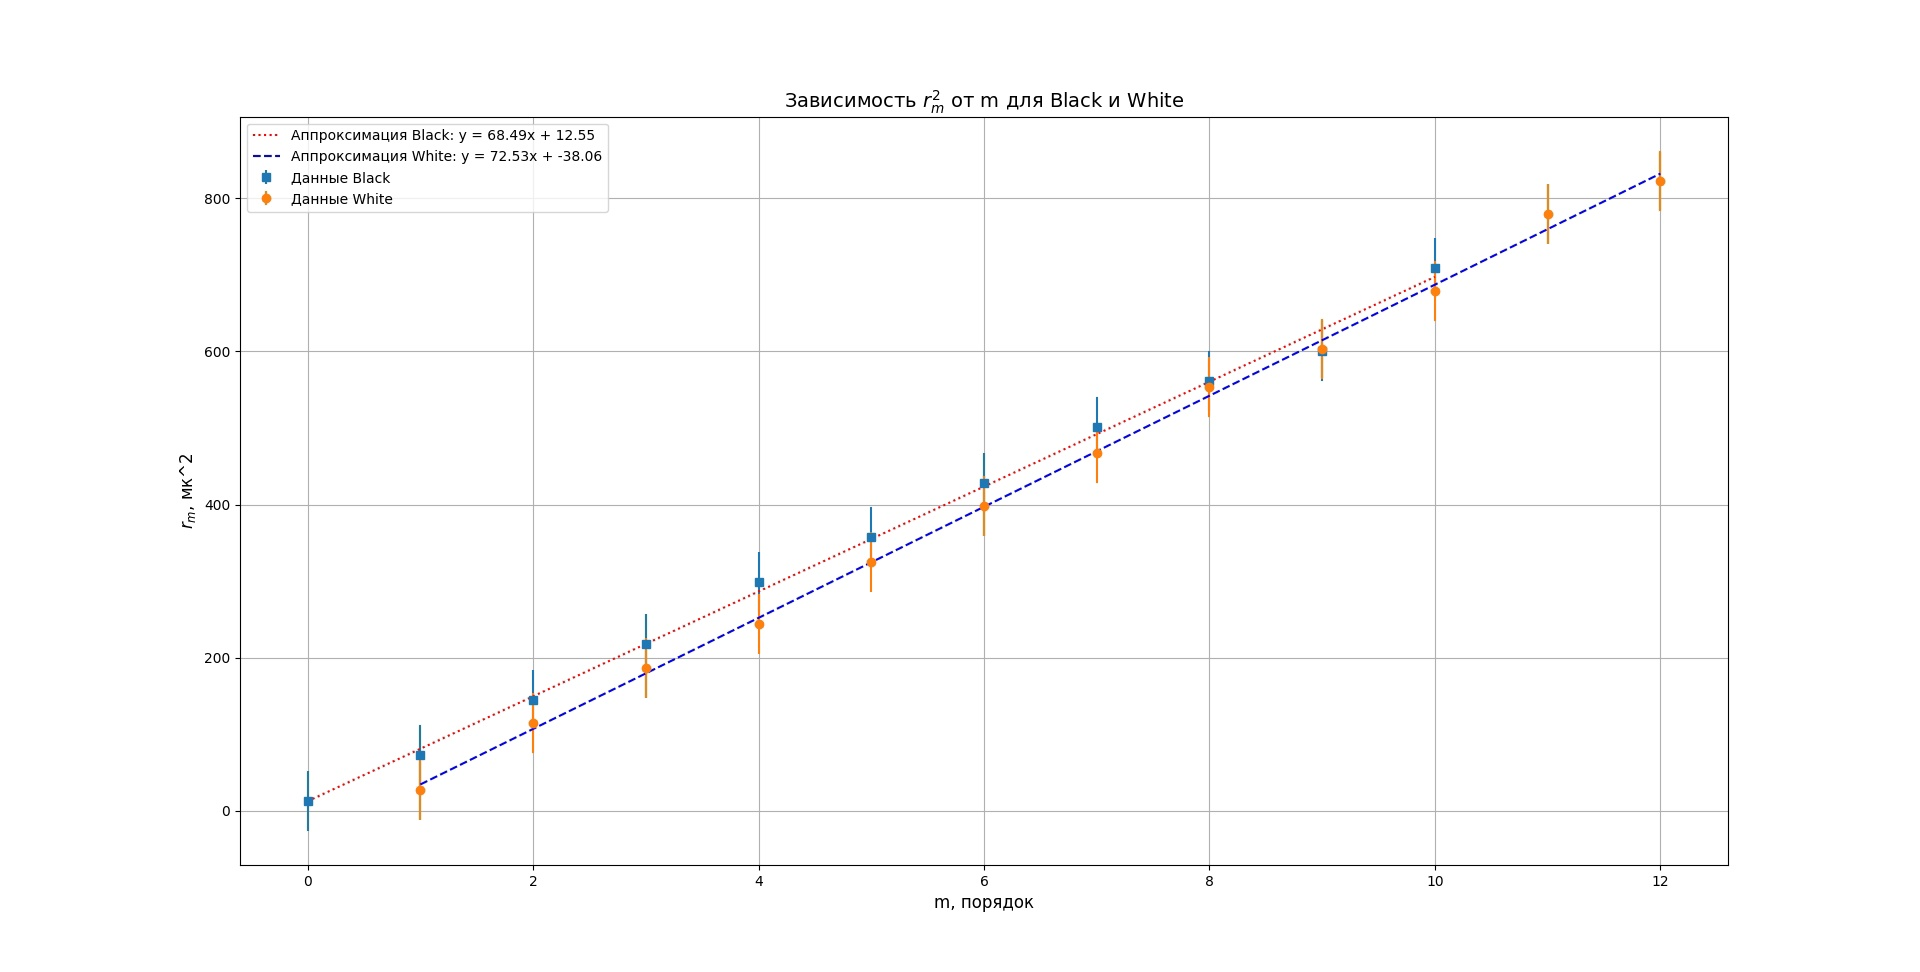
\includegraphics[width=0.9\textwidth]{график2.jpg}
   \caption{Кольца Ньютона для двух длин волн}
   \label{ringImage}
\end{figure}
На графике представлена зависимость квадрата радиуса кольца $r_m^2$ от его номера $m$. Методом наименьших квадратов определены:
\begin{itemize}
    \item коэффициент наклона $k = 2R\lambda = 70,51 \pm 1,29$ мк$^2$;.
\end{itemize}
можно определить радиус кривизны линзы $R$:
$$
R = \frac{k}{\lambda} = 1,3 \pm 0,0024 \text{мм}
$$


В ходе опыта с двухполосным фильтром (см. рис. \ref{ringImage}) было установлено, что тёмные полосы двух интерференционных картин точно совпадают через $\Delta m = 15$ полосы. Из формулы получаем соотношение:
$$
\frac{\Delta m - 1}{\Delta m} = \frac{\lambda_1}{\lambda_2} = \frac{}{} \approx 0.93.
$$
С использованием указанных значений $\lambda_1$ и $\lambda_2$ получается значение $\lambda_1/\lambda_2 = 0.94$, что практически совпадает с полученным значением.

\section{Выводы}
В ходе лабораторной работы познакомились с явлением интерференции в тонких пленках на примере колец Ньютона и с методикой интерференционных измерений кривизны стеклянной поверхности.
Был построен график зависимости $r_{m}^{2}(m)$ и $r_{m}'^{2}(m)$ из которых были получены коэффициенты наклона. По этим коэффициентам наклона, зная длиину волны был получен радиус кривизны поверхности.
Также были проведены наблюдения биений из которых мы получили, что темные полосы двух интерференционных картин точно совпадают через dm = 15 полос.
\end{document}